This section is based on information from the book AI techniques for game programming\cite{buckland2002ai} chapter 7, 8 \& 9 and from the book Neural networks: a systematic introduction\cite{rojas1996neural} chapter 7.
\\[0.5cm]
Neural networks are models that imitate the brains behavior and have been created as an option to model artificial intelligence and analyze machine learning. The human brain is made up of billions of neurons that are interconnected in a big grid where they communicate by firing electrical shocks through the network of neurons. The human brain is extremely complex and can calculate vast amounts of data in no time. This is why scientists and mathematicians have been trying to emulate this behavior to create artificial intelligence.

\begin{figure}[!ht]
\centering
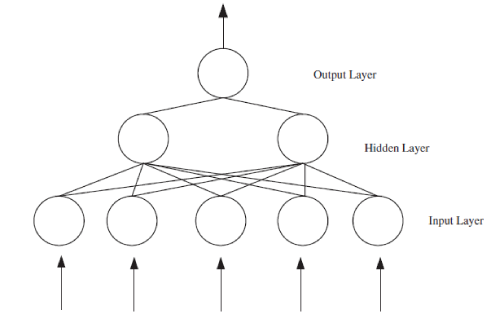
\includegraphics[width=0.8\linewidth]{billeder/ANN.png}
\caption{A simple neural network with 3 layers. \cite{stockForecasting}}
\label{fig:ANN}
\end{figure}

Artificial neural networks (ANN) are artificial neurons (nodes) that are connected in a network. The network consists of an arbitrary number of layers that are interconnected. The most common structure in these networks are a feed forward structure. This kind of structure has the characteristic that it only flows data from the input layer through the hidden layers to the output layer. There are no loops in the network thus making it unable to reiterate any information. Normally all of the nodes in the input layer is connected to all of the nodes in the second layer. The same connections are done in the next layers until we hit the output layer. This will give us the sum($\sum_{i=0}^{i=n+1} w_i x_i$) of all the previous nodes($x_i$) and their weights($w_i$) in every node in the next layer (see Figure~\ref{fig:weight_of_layers}).
\begin{figure}[!ht]
\centering
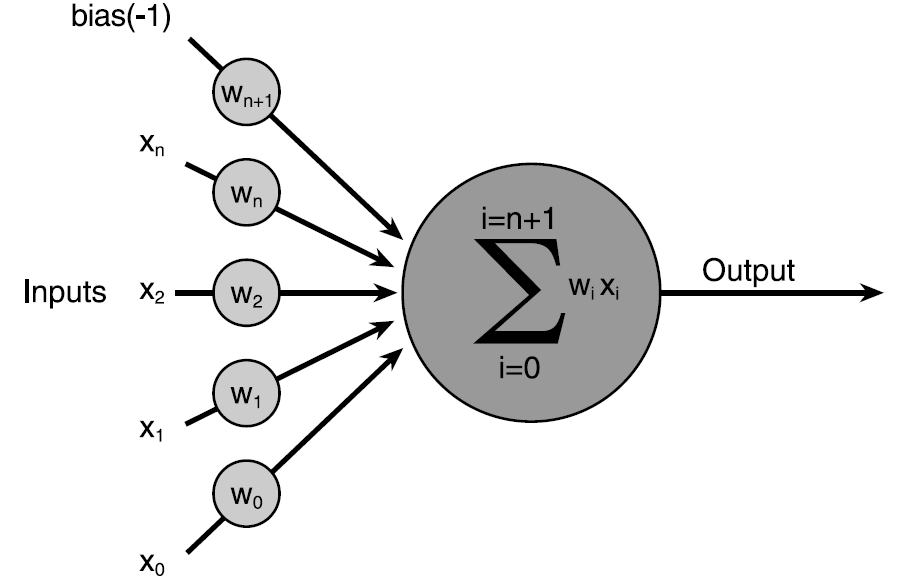
\includegraphics[width=0.8\linewidth]{billeder/weight_of_layers.png}
\caption{How the weight is calculated from one layer to the next. \cite[P. 251]{buckland2002ai}}
\label{fig:weight_of_layers}
\end{figure}
All of these connections carry a weight that dictates how data flows through the network and reflects the relationship between the inputs and the outputs of the network. The inputs of the network should be all the factors that has an influence on the output that we want to approach. As an example for the electricity price we would want to input weather data, temperature, demand, availability etc. \cite{21} to get the price as an output from the network. 

Every node in our network contains an activation function. This function (when calculated) tells us whether the artificial neuron should fire or not, i.e. if the neuron should transmit the data from the current layer to the next layer. There are a lot of different activation functions with the simplest form being the binary step function that either fires or not. This depends on the input and gives us a low threshold of complexity which is good in simple neural networks as the relations between the nodes do not need to be that fine grained. In more complex systems we want activation functions with a broader output range than binary. In many cases a sigmoid function is used as the activation function. This is because of the ''S''-shape that enables it to compute outputs in a non-linear way. The non-linear nature of the sigmoid functions is what makes the neural network able to compute non-trivial problems in reasonable sized networks. The sigmoid function allows the activation functions of the neurons to have a broader range of inputs which will produce an output compared to step activation functions. To be able to calculate a non-trivial problem in these kind of networks we need what is called a training algorithm. This algorithm depicts how the network evolves over time also known as learning. There are two kinds of learning; unsupervised learning and supervised learning.

\subsection{Unsupervised learning}
Unsupervised learning is the problem of identifying structure in the underlying data, i.e. we do not have the specific outputs for the input data. Instead we have a problem where we want the neural network to try and estimate some behaviour relative to a specific task based on assumptions we have about the system it performs on. It is commonly used with estimation problems like "Cluster Analysis" that in short is an attempt to find matching criterion in data and group the data in clusters. This is often done by exploring the dataset and that is what unsupervised learning is good for. It also works with Artificial Intelligence(AI) that have to explore parts of the (virtual)world. In \cite{buckland2002ai} he explains how an unsupervised learning feed-forward artificial neural network trains itself using a genetic algorithm to keep track of the fitness function of the AI. The fitness function is used to inform the AI if it is doing good or bad according to requirements established before the experiment. This fitness function is what trains the network where the AI will get a plus score if it encounters what we are looking for and get negative if it hits something that we defined as "wrong". Based on this fitness function it will update the weights of the neural network accordingly to what is most beneficial for the network as a total. After it has been allowed to do a lot of runs it begins to get a sense of what it is exploring and should be able to make better choices for each run.

\subsection{Supervised learning}
Supervised learning are a set of algorithms that use a dataset which contains both the inputs and outputs. This dataset is used to train the Artificial Neural Network to make it able to do calculations on current data and predict the outcome. An example of an algorithm used for supervised learning is the Backpropagation algorithm. 
It starts out by randomly assigning weights to all of the connections between the neurons. It then calculates the output of the network and compares it to the expected output. From the comparison of input and expected output it calculates the error margin and adjusts the weights accordingly. This is done for all the hidden layers until we hit the input layer. All of these steps are called an epoch. We will repeat as many epochs as we need until the sum of all the errors are within a given threshold. The name of the algorithm originated from these epochs where it propagates the error backwards in the network. We use Resilient Bacpropagation (RPROP) which is based on the traditional Bacpropagation algorithm as described in \cite{rpropForGeometricDilution,adaptiveRprop}. It is an algorithm that is better at escaping local minima and at the same time scales linearly to the number of input parameters. In short, the difference is in how the weights are being updated through evaluating the behaviour of the error function. The traditional Backpropagation adjusts its weights based on the actual value of the derivative and since the derivative value decreases exponentially as further it gets from the output layer it will take longer time for the last neurons to learn. In RPROP the derivative sign decides the weight adjustment and not the magnitude of the derivative as with traditional Backpropagation. RPROP use the same amount of computational effort but is faster due to the derivative sign evaluation. Furthermore, it is not necessary to define the learning rate or momentum because they are automatically adapted and therefore we avoid spending time on fine-tuning these parameters.

Supervised learning can be thought of as learning with a teacher. As an example we can use the XOR table:

\begin{table}[H]
\centering  % used for centering table
\begin{tabular}{c c c} % centered columns (3 columns)
Input \#1 & Input \#2 & Output \\ [0.5ex] % inserts table 
%heading
\hline                  % inserts single horizontal line
0 & 0 & 0  \\ % inserting body of the table
1 & 0 & 1  \\
0 & 1 & 1  \\
1 & 1 & 0 \\ [1ex] % [1ex] adds vertical space
\hline %inserts single line
\end{tabular}
\caption{This training set is very simple yet it illustrates a training set for a supervised learning algorithm very well.} % title of Table
\label{table:xor-table} % is used to refer this table in the text
\end{table}

In this dataset we are given the inputs together with the expected output. The output gives the Bacpropagation algorithm a direction to follow when minimizing the error function (based on the inputs) of the network. It is possible because the predicted output is known in advance and the inputs cannot therefore be directly compared to it. The comparison allows the network to calculate the direction that the error correction should take to approach the best possible prediction. Also the sigmoid activation function helps the network in approaching the target output since the sigmoid function always has a positive derivative that ensures a direction to follow\cite[p. 153]{rojas1996neural}. The direction given by the sigmoid function will point us towards the global minimum of the approached function, i.e. a small value is equal to a small error. The inputs and the associated outputs are given when considering Table~\ref{table:xor-table}, e.g. input 1 and 0 is expected to output 1. The neural network will initialize weights and start to run the Bacpropagation. The Bacpropagation algorithm will compare the output it predicts to the expected output, e.g. we may get an output of 0.5 from the network (based on the random weight initialization) and this is compared to the expected output 1. Because of the sigmoid function we know what direction the weights should be corrected to come closer to the output of 1 --- as an example, the network identifies that the weight for input 0 should be approaching 0 and the weight for 1 should be approaching one in order to obtain 1 as output. This allows the Bacpropagation algorithm to recalculate the weights and be sure that it is heading for the global minimum of the error function thus heading for the right output.
%[FORKLAR MATEMATIKKEN EVT MED EKSEMPEL s. 332 i bogen]

In Artificial Neural Networks the bias neurons are often added to the layers to help them learn. The bias neurons are added to give the activation functions the ability to change its output even if x is zero. If we look at the graph in figure ~\ref{fig:activationFunctions} it uses the following activation function: \begin{math} \frac{1}{(1+e^{(-cx)})} \end{math} where c is the weight. A problem that is seen from the figure is how values from 0-2 cannot result in an output below 0,5, e.g. if the function has an input value of 1 then the weights can never be adjusted enough to get the function below 0,5.

\begin{figure}[!ht]
\centering
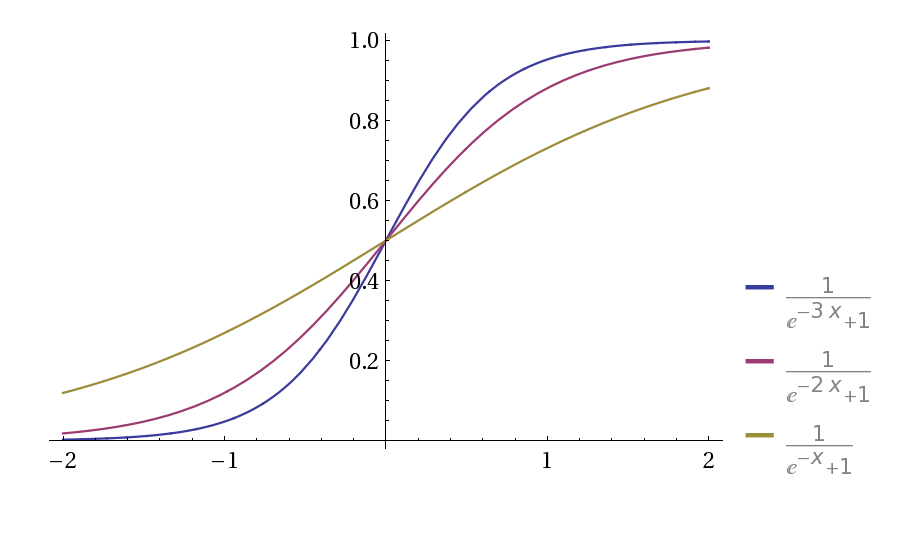
\includegraphics[width=0.8\textwidth ,natwidth=410,natheight=237]{billeder/ActivationFunctions.png}
\caption{Activation functions with different weights}
\label{fig:activationFunctions}
\end{figure}

The figure shows how the gradient of the function alters with different weight values. Even though the gradient of the function is clearly altered by the weights the function is still outputting the same result for zero thus we cannot alter the output for x equal to zero just by altering the weights. This is what we use the bias for. If we apply a \fnurl{bias}{http://en.wikipedia.org/wiki/Inductive_biasrks} of one to all of the neurons we will be able to shift it either to the left or the right. In figure ~\ref{fig:activationFunctionsWithBias} we see the same function as before where the weight is set to 2. The difference is that we added a bias (b) to this function: \begin{math} \frac{1}{(1+e^{(-2x+b)})} \end{math} \cite[p. 165]{rojas1996neural}

\begin{figure}[!ht]
\centering
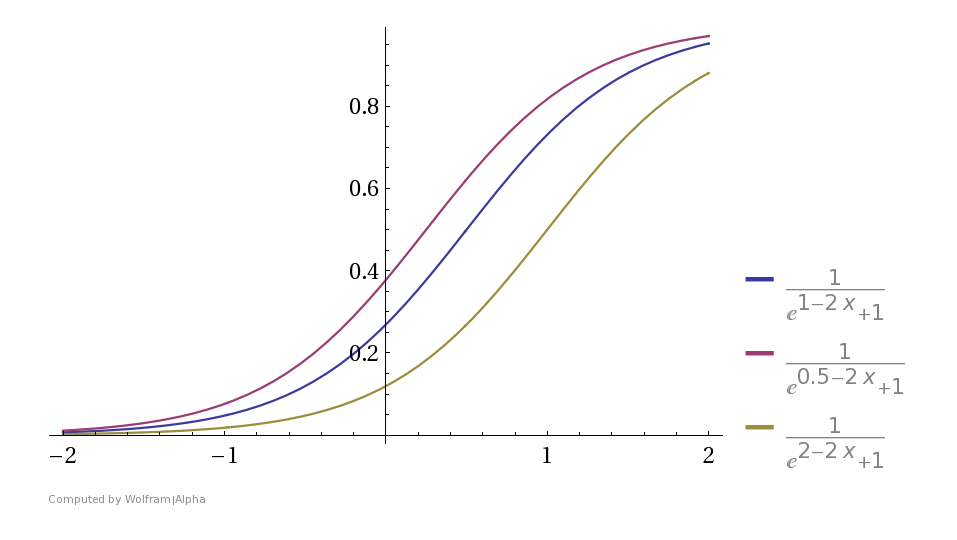
\includegraphics[width=0.8\textwidth ,natwidth=410,natheight=237]{billeder/ActivationFunctionsWithBias.png}
\caption{}
\label{fig:activationFunctionsWithBias}
\end{figure}

\subsection{Common pitfalls}
\label{sec:ANNCommonPitfalls}
When we are trying to fit our algorithm and make it recognize patterns we will encounter several possible pitfalls. First of all there is the chance of ending up in a local minima. This is when the the Bacpropagation algorithm attempts to find the global minimum of the error curve thus having reduced the error as much as possible. The algorithm works by trying to reduce this error margin a little step at a time. If it encounters a local minimum on the curve and thinks it has reached the global minimum it gets stuck and we will get an inaccurate result that can be seen in Figure~\ref{fig:localMinimum}. To avoid the Backpropagation algorithm to falsely accept a local minimum as the global minimum we can give the algorithm momentum. This is done by adding a bit of the last error correction from the earlier layer to the next layers error correction. This way the algorithm will move right past small deviations in the error correction face.

\begin{figure}
\centering
\begin{minipage}{.5\textwidth}
  \centering
  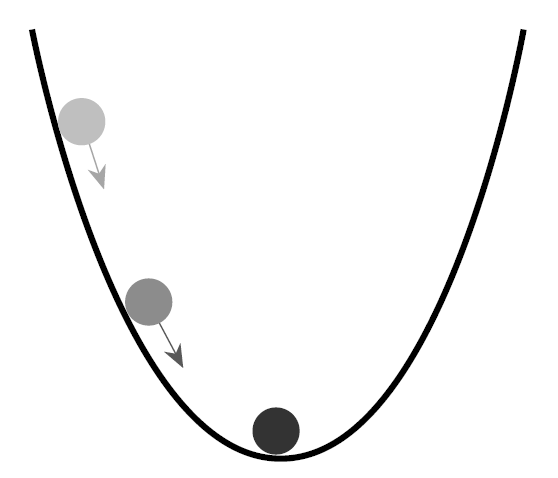
\includegraphics[width=.4\linewidth]{billeder/globalMinimum.png}
\end{minipage}%
\begin{minipage}{.5\textwidth}
  \centering
  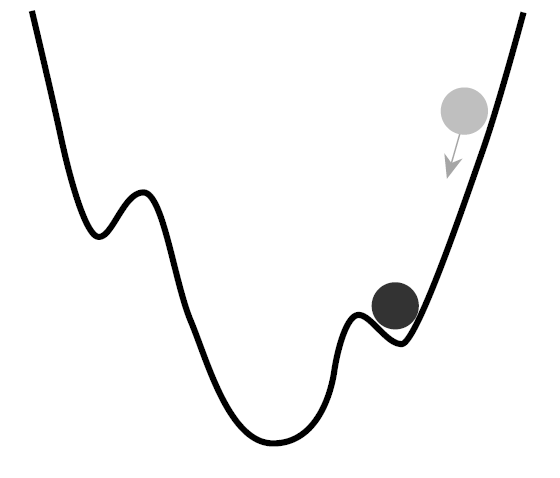
\includegraphics[width=.4\linewidth]{billeder/localMinimum.png}
\end{minipage}
\caption{The first figure shows a global minimum whereas the second shows a local minimum \cite[P. 318]{buckland2002ai}}
\label{fig:localMinimum}
\end{figure}

Another pitfall when working with neural networks is overfitting the algorithm. This is when the algorithm instead of finding a generalized pattern in the inputs it will find an over-fit pattern that will fit exactly the input resulting in problems when presenting the network for unseen data. This is better shown in Figure~\ref{fig:overfitting}.
\begin{figure}[!ht]
\centering
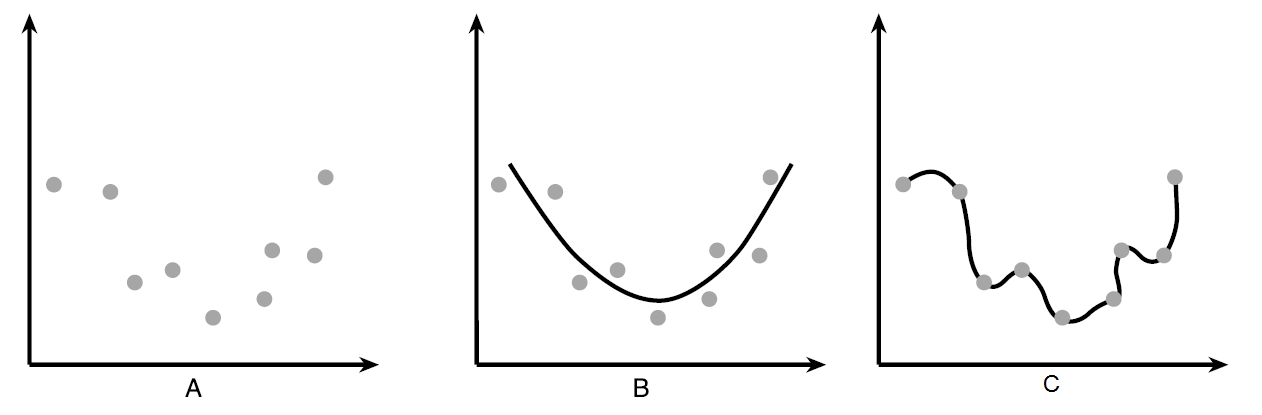
\includegraphics[width=0.8\linewidth,natwidth=1262,natheight=415]{billeder/overfitting.png}
\caption{A. The plot graph of the input B. The generalized function C. An over-fit function \cite[P. 319]{buckland2002ai}}
\label{fig:overfitting}
\end{figure}
This can be avoided by some simple techniques. First of all we want to reduce the neurons as much as possible as long as it does not interfere with our performance of the system (also known as pruning). This is a trial and error problem and has to be tweaked along with evolving the neural network. Another option is to add noise to avoid this problem. By adding noise(random data values) we prevent the algorithm from fitting the function to closely to the given data. Thus giving us a more generalized function where it hopefully will be able to give a better result on unseen data. Early stopping is another method to avoid over-fitting. This is only possible with large datasets where you can split it into two equal datasets where the first will work as a training set and the second will work as a validation set. We will keep training the dataset and checking with the validation set until the difference between those two start to increase.

\subsection{Summary}
This section touched the basics of neural networks and where the inspiration for these networks came from. Feed-forward was presented as the most common architecture used for Artificial Neural Networks and it will also be applied in this thesis. This architecture allows data to only flow from input to output with no loops in it. We elaborated on what activation functions that exist and how they are used in neural networks. Since neural networks are all about the computer learning to calculate complex problems it requires a learning algorithm. Unsupervised learning is obtained by exploring possibilities in a given domain and approaching goals that have been defined, i.e. it is based on some predefined assumptions about what to explore. It has no definitive goal (opposed to supervised learning) but a success factor that it tries to maximize. Supervised learning (as used in this thesis) attempts to learn by trial and error until it satisfies an error margin or after a predefined number of epochs. The learning is achieved by comparing actual inputs to their outputs, i.e. we get a direction to follow by comparing the two.

There are some common pitfalls to be aware of when modelling an Artificial Neural Network. Among these are over-fitting of the function that we are trying to achieve. The result is a function that only fits on the trained data and not data that has never seen before --- the purpose of Machine Learning is to generalize beyond the training set as described in Section~\ref{sec:machineLearning}. Another issue is when the algorithm falsely believes that a local minimum is the global minimum and thereby obtains a faulty result. Both of these concerns must be considered when modelling our Artificial Neural Network.

The focus of this thesis is the use of a Feedforward Neural Network with Resilient Backpropagation and therefore the main focus has been the supervised training. In this context the importance of the dataset must be emphasized because it is what ensures accuracy of our ANN. The training set has to be developed and refined during a training period of a network and relies a lot on experience and tinkering with the inputs. We need to normalize the dataset to fit the activation function. The influential inputs must be discovered through comprehensive analysis and we must investigate the best representation of them.